% ==================================================================================================
\subsection{Homogenizing Effect of Turnover}\label{aa:homogenize}
\begin{figure}[H]
  \centering
  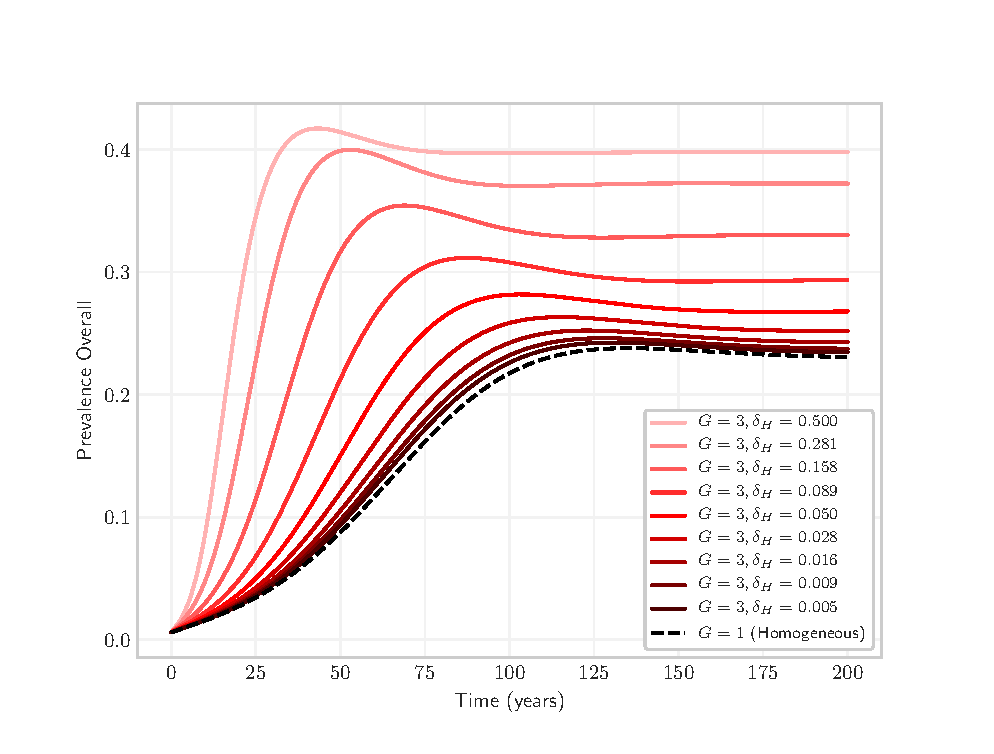
\includegraphics[width=0.6\linewidth]{vary-zeta-prevalence-[0005,05].eps}
  \caption{Overall prevalence predicted by a heterogeneous system
    under a wide range of high turnover rates.
    Note how the heterogeneous system ($G = 3$) converges on a homogeneous system ($G = 1$)
    with very high turnover rates (duration $\delta_H$ approaches zero).}
  \label{fig:prev-converge}
\end{figure}
% ==================================================================================================
\subsection{Infection Convection}\label{aa:new-inf}
\begin{figure}[H]
  \centering
  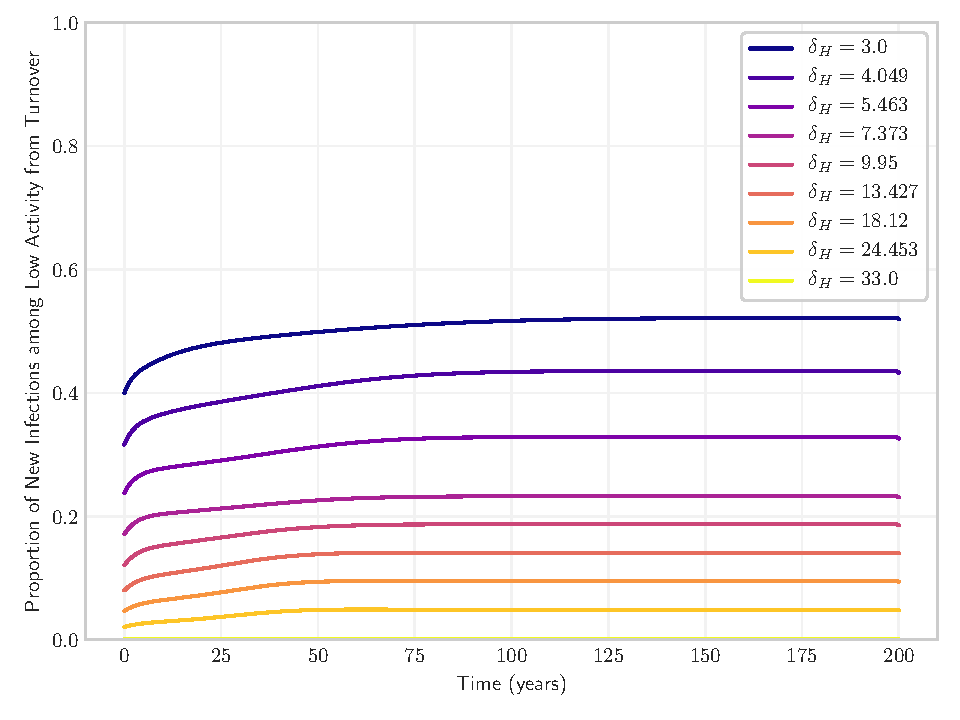
\includegraphics[width=0.6\linewidth]{compare-turnover-newinf-L.pdf}
  \caption{Proportion of new infections among the low risk group
    which represent turnover of infected individuals
    versus infection of individuals in the low risk group ($\delta_I = 10$ years).
    At high levels of turnover, an notable proportion of prevalence
    in the low risk group can be attributed to turnover of infected individuals
    from higher risk groups.}
  \label{fig:new-inf-L}
\end{figure}